\documentclass[12pt]{report}

\usepackage[T1]{fontenc}
\usepackage[utf8]{inputenc}
\usepackage{graphicx}

\begin{document}
{\Large \textbf{Giro de un motor de corriente directa.}\\}
\Large{Enesto Alonso Partida López\\ Universidad Politecnica De La Zona Metropolitana De Guadalajara\\ Mecatronica 4 A\\ Septiembre-diciembre 2019}\\
{10 de octubre 2019 }\\

\begin{center}

\includegraphics[scale=1]{../../../Downloads/upzmg.jpg} \\
\end{center}

\newpage
{\huge \textbf{¿Que es un motor de corriente directa?}\\}


{\Large Los motores de Corriente Directa o motor DC(correspondiente a las iniciales en inglés “direct current”) es también conocidos como motor de Corriente Continua o motor CC. }\\

\begin{figure}[hbtp]
\caption{Motor de CD}
\centering
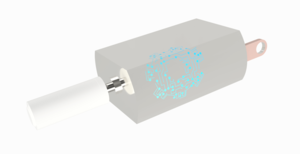
\includegraphics[scale=0.5]{../EV_2_4_giro_de_un_motor_de_corriente_directa/motor+dc.png}
\end{figure}

{\huge \textbf{¿Comó se clasifican los motores?}\\}
\begin{itemize}
\item Imán permanente
\item Devanado shunt 
\item Devanado serie
\item Devanado compuesto 
\end{itemize}
\newpage

{\huge \textbf{Curva de toque y velocidad}\\}\\
{\Large Para un dado torque proporcionado por el motor, se puede utilizar la curva corriente-torque para determinar la corriente requerida cuando se le aplica el voltaje nominal al motor.  
Como regla general, los motores generan grandes torques a baja velocidad, y grandes torques implican una demanda mayor de corriente por parte del motor.\\
El torque de arranque o torque crítico (Ts): Es el torque máximo que puede proporcionar un motor a velocidad cero, asociado con el arranque o sobrecarga del motor.\\
La velocidad de no carga Wmáx: Es la máxima velocidad sostenida que puede lograr el motor. Esta velocidad sólo se puede lograr cuando no se aplica carga o torque al motor.
}\\
\\\begin{figure}[hbtp]
\caption{Curva de toque-velocidad}
\centering
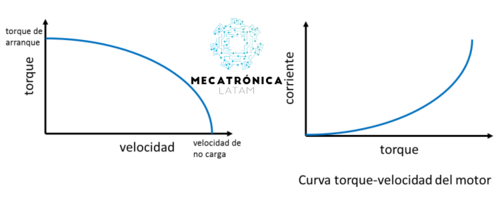
\includegraphics[scale=0.5]{../EV_2_4_giro_de_un_motor_de_corriente_directa/image4526.png}
\end{figure}
\newpage

{\huge \textbf{Motores se imán permanente }\\}\\

{\Large El motor de imán permanente es ideal en aplicaciones de control por computadora debido a su linealidad torque-velocidad, aunque únicamente se utilizan en aplicaciones de baja potencia pues su potencia nominal usualmente se limita a 5 hp (3278 W) o menos.}\\
\begin{figure}[hbtp]
\caption{Motor de imán permanente}
\centering
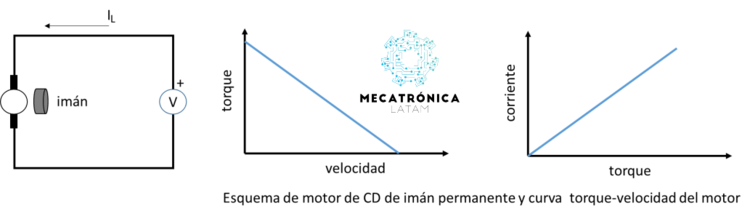
\includegraphics[scale=0.5]{../EV_2_4_giro_de_un_motor_de_corriente_directa/curva-motor-de-iman-permanente.png}
\end{figure}


{\huge \textbf{Motores Shunt }\\}\\

{\Large Los motores shunt presentan velocidad casi constante sobre un gran rango de carga, cuentan con un torque de arranque de aproximadamente 1.5 veces el torque operativo nominal, tienen torque de arranque más bajo que cualquiera de los motores de CD y se puede convertir económicamente para permitir una velocidad ajustable al colocar un potenciómetro en serie con los devanados de campo.}\\
\begin{figure}[hbtp]
\centering
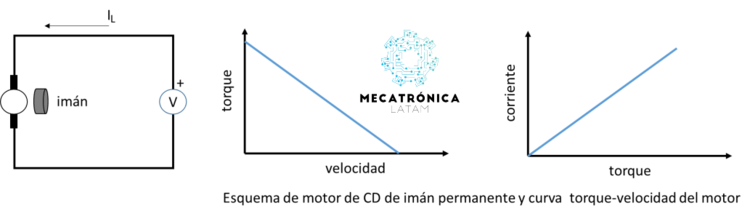
\includegraphics[scale=.5]{../EV_2_4_giro_de_un_motor_de_corriente_directa/curva-motor-de-iman-permanente.png}
\caption{Motor Shunt}
\end{figure}


{\huge \textbf{Motores Serie }\\}


{\Large  Los motores en serie generan torques de arranque muy altos, velocidad extremadamente variable dependiendo de la carga, y gran velocidad cuando la carga es pequeña y ademas los motores en serie grandes pueden fallar catastróficamente cuando se descargan súbitamente debido a la fuerza dinámica a altas velocidades, a esto se le llama sin control. }\\
\begin{figure}[hbtp]
\centering
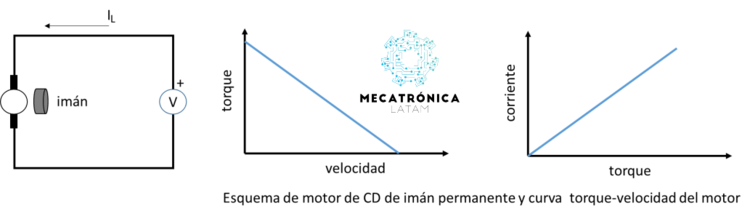
\includegraphics[scale=0.5]{../EV_2_4_giro_de_un_motor_de_corriente_directa/curva-motor-de-iman-permanente.png}
\caption{Motor Serie}
\end{figure}

\newpage
{\huge \textbf{Motores Compuestos }\\}


{\Large  La velocidad máxima de un motor compuesto es limitada, su regulación de velocidad no es tan buena como la de un motor en derivación. El torque producido por los motores compuestos es un poco menor que el de los motores en serie de similar tamaño. }\\ \\
\begin{figure}[hbtp]
\centering
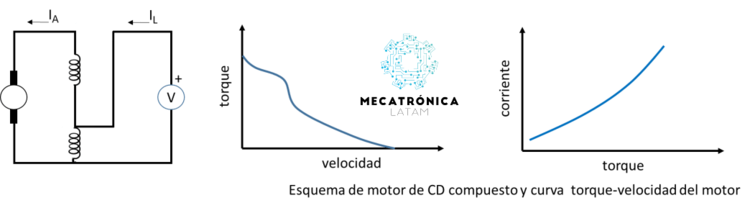
\includegraphics[scale=0.5]{../EV_2_4_giro_de_un_motor_de_corriente_directa/curva-motor-compuesto.png}
\caption{Motor Compuesto}
\end{figure}

\newpage
{\huge \textbf{Bibliografia:}\\}\\
{\large
@online{Electronica Unicrom,
author = {Mecatronica},
title = {Motor de Corriente Directa DC o Continua CC},
year = {2018},
url = {https://www.mecatronicalatam.com/motores/motores-de-cd},
OPTsubtitle = {Motores
OPTversion = {copyright},
OPTdate = {2},
OPTmonth = {6},
OPTurldate = {http://arteymedios.org/tutoriales/item/76-controlar-motores-de-corriente-continua-con-puente-h},
}
}

\end{document}